\documentclass[a4paper,12pt]{article} %{report}
\usepackage{amsmath}
\usepackage{graphicx}
\usepackage{float}
\usepackage{bm}
\usepackage{verbatim}
\usepackage{fixmath} %mathbold
\usepackage{amssymb}
\usepackage{indentfirst}
\usepackage[utf8]{inputenc}
\usepackage{xcolor}
\usepackage[colorlinks=true]{hyperref}
\hypersetup{colorlinks,citecolor={green!70!black},filecolor=magenta,linkcolor={red!50!black},urlcolor=cyan}
\addtolength{\textheight}{6cm} %aumenta o espaço vertical do corpo do texto   6
\addtolength{\voffset}{-3.5cm} %começa a escrever mais em cima na página      -3.5
\addtolength{\textwidth}{6cm} %aumenta o espaço horizontal do corpo do texto  6
\addtolength{\hoffset}{-3cm} %começa a escrever mais a esquerda na página     -3
\setlength\arraycolsep{1.3pt} %reduz espaços quando usar & = &
\newcommand{\brel}{{\bm b}_{rel}}
\newcommand{\pt}{{\bm p}_{t}}
\newcommand{\rr}{{\bm r}}
\newcommand{\qq}{{q\bar q}}

\begin{document}
\begin{center}
\begin{flushleft}
 \textcolor{red}{\today}
\end{flushleft}
\vspace{-0.95cm}
\begin{flushright}
  \textcolor{red}{\textbf{lambda 01}}
\end{flushright}
\vspace{0.2cm}

%\texttt{Artigo base:}
%\textbf{Target Fragmentation in $\mathbold{pp}$, $\mathbold{ep}$ 
%and $\mathbold{\gamma p}$ Collisions at High Energies}\\
%\textit{U. D'Alesio and H.J. Pirner}\\
%\href{https://arxiv.org/abs/hep-ph/9806321v3}{arXiv:9806321v3 [hep-ph] 26 Jan 2000}
\end{center}

\section{Introdução}
\indent Em artigos anteriores nós propomos a utilização do formalismo de dipolos de cor 
para descrever a produção de partículas dominantes em espalhamento fóton-próton, 
em processos inclusivo e exclusivo.

Em um primeiro momento, motivados por dados experimentais daquela época (2015), 
focamos na produção de nêutron dominante em colisões elétron-próton.

Em um segundo momento, aplicamos o mesmo formalismo para descrever a produção de delta dominante, 
que por sua vez pode decair em nêutron e dessa forma popular o espectro de nêutron dominante. 
Além disso, nós também estendemos o formalismo para descrever colisões hádron-hádron ultraperiféricas, 
nas quais um dos hádrons atua como fonte de fótons.

No presente trabalho objetivamos (inicialmente) aplicar o mesmo formalismo para descrever a produção 
de lambda dominante. Neste caso o próton inicial decai no par káon + lambda 
$(p \rightarrow K^{+}+\Lambda^{0})$, com posterior interação entre o káon e o dipolo de cor 
(flutuação do fóton emitido pelo elétron/hádron inicial).

A motivação para tal análise é a possibilidade de medida da produção de lambda dominante no JLab. 
Além disso, uma vez que os canais de decaimento do $\Lambda^{0}$ são $\Lambda \rightarrow p + \pi^{-}$
e $\Lambda^{0} \rightarrow n + \pi^{0}$, esse processo também pode contribuir no espectro de nêutron 
dominante que nós temos estudado nos últimos anos.

Nota 1: investigar se essa última parte faz sentido.

Nota 2: se o pico do espectro de lambda for muito abaixo de $x_L=0.8$, 
é possível que a fatorização $\sigma(\gamma p)= f_{K/p}\times \sigma(\gamma K)$
não seja mais válida.


\newpage
\section{Formalismo (inclusivo)}
\begin{figure}[!h]
 \centering
 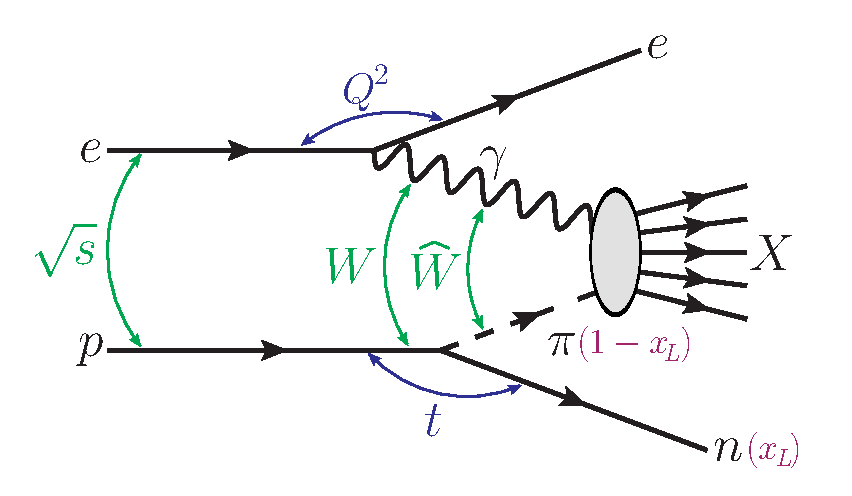
\includegraphics[scale=0.65]{../figures/diagrams/ln_inc}
 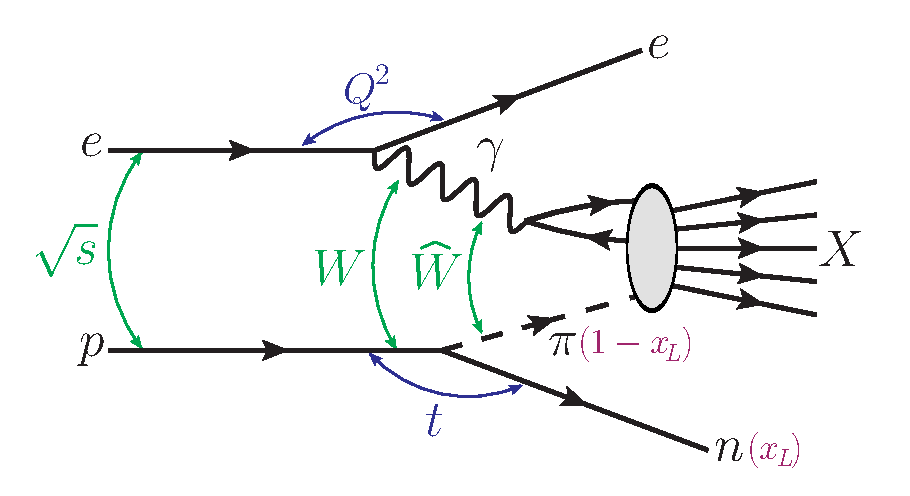
\includegraphics[scale=0.65]{../figures/diagrams/ln_inc_dip_tese}
 \caption{Produção de nêutron dominante (esquerda) no formalismo de dipolo de cor (direita).}
 \label{fig:ln_inc}
\end{figure}

Em altas energias a produção de nêutron dominante em um espalhamento
fóton-próton (Fig.\ref{fig:ln_inc} , painel esquerdo) é descrita pela
seguinte seção de choque diferencial:
\begin{eqnarray}
  \frac{d^2\sigma(W, Q^2, x_L, t)}{dx_Ldt} = 
  f_{\pi/p}(x_L, t) \times \sigma_{\gamma^*\pi^*}(\hat{W}^2, Q^2)
\end{eqnarray}
tal que $f_{\pi/p}(x_L, t)$ é o fluxo de píons emitido pelo próton
e $\sigma_{\gamma^*\pi}(\hat{W}^2, Q^2)$ é a seção de choque
fóton-píon. 
As quantidades envolvidas podem ser visualizadas na Fig.\ref{fig:ln_inc}.
A energia de centro de massa do sistema fóton-píon ($\hat W$)
é descrita em termos da energia de centro de massa do sistema fóton-próton ($W$)
e da fração de momentum do próton portada pelo nêutron ($x_L$):
\begin{eqnarray}
  \hat W^2 = (1-x_L)W^2\,.
\end{eqnarray}
Em termos de quantidades mensuráveis, a virtualidade do píon ($t$)
é dado por
\begin{eqnarray}
  t \simeq -\frac{p_T^2}{x_L} - \frac{(1-x_L)(m_n^2 - m_p^2x_L)}{x_L}\,
\end{eqnarray}
onde $p_T$ é o momentum transverso do nêutron.\\
\indent No formalismo de dipolo de cor o processo descrito acima
pode ser descrito em termos dos seguintes subprocessos
(Fig. \ref{fig:ln_inc}, painel direito):\\
\hspace*{1cm} [1]: O fóton (emitido pelo elétron) flutua em um par quark-antiquark (dipolo de cor, $\qq$);\\
\hspace*{1cm} [2]: O próton decai pelo canal $p\rightarrow \pi^{+}+n$, dando origem ao nêutron dominante;\\
\hspace*{1cm} [3]: O píon do decaimento do próton interage com o dipolo de cor ($\qq + \pi \rightarrow X$).\\

\subsection{Fluxo de píons}
O fluxo de píons $f_{\pi/p}(x_L, t)$ (função de desdobramento)
é descrito por
\begin{eqnarray}
  f_{\pi/p} (x_L,t)  = 
  \frac{1}{4 \pi} \frac{2 g_{p \pi p}^2}{4  \pi} 
  \frac{-t}{(t-m_{\pi}^2)^2} (1-x_L)^{1-2 \alpha(t)}  
  [F(x_L,t)]^2
\end{eqnarray}
sendo $g_{p \pi p}^2/(4\pi)=14.4$ a constante de acoplamento
$\pi^0pp$ e $\alpha(t)$ está relacionado com a trajetória 
de Regge do píon $\alpha(t)_{\pi}$.
Para descrever o fator de forma $[F(x_L,t)]$ utilizaremos diferentes modelos:
\begin{eqnarray}
  F_1(x_L,t) &=& \exp \left[ R^2 \frac{(t-m_{\pi}^2)}{(1-x_L)} \right], 
  \hspace{0.5cm} \text{com } \alpha(t) = 0 
  \text{ e } R = 0.6 \text{ GeV}^{-1}.\\
  F_2(x_L,t) &=& 1, 
  \hspace{0.5cm} \text{com } \alpha(t) = \alpha(t)_{\pi} \simeq t.\\
  F_3(x_L,t) &=& \exp \left[ b (t-m_{\pi}^2) \right],
  \hspace{0.5cm} \text{com } \alpha(t) = \alpha(t)_{\pi} \simeq t
  \text{ e } b = 0.3 \text{ GeV}^{-2}.\\
  F_4(x_L,t) &=& \frac{\Lambda_m^2-m_{\pi}^2}{\Lambda_m^2-t},
  \hspace{0.5cm} \text{com } \alpha(t) = 0 
  \text{ e } \Lambda_m = 0.74 \text{ GeV}.\\
  F_5(x_L,t) &=& \left[\frac{\Lambda_d^2-m_{\pi}^2}{\Lambda_d^2-t}\right]^2,
  \hspace{0.5cm} \text{com } \alpha(t) = 0 
  \text{ e } \Lambda_d = 1.2 \text{ GeV}.\\ 
\end{eqnarray}.  
\end{document}


